\documentclass[aspectratio=169]{beamer}
\usetheme{Madrid}
\usepackage[utf8]{inputenc}
\usepackage[T1]{fontenc}
\usepackage{tikz}
\usepackage{amssymb}
\usepackage{graphicx}
\setbeamertemplate{navigation symbols}{}
\setbeamercolor{title}{fg=white,bg=teal!60!black}
\setbeamercolor{frametitle}{fg=white,bg=teal!60!black}
\setbeamercolor{block title}{bg=teal!60!black!20,fg=black}
\setbeamercolor{block body}{bg=teal!60!black!8,fg=black}
\setbeamercolor{item}{fg=teal!60!black}
\setbeamercolor{itemize item}{fg=teal!60!black}
\setbeamertemplate{itemize item}[triangle]

\title{Computer Basics 4 — Phishing \& Fake Logins}
\subtitle{A fake domain looks ALMOST right — spot the exact difference}
\author{ByteForge --- Grade 7 --- Game Maker}
\date{}

\begin{document}

\begin{frame}
    \titlepage
\end{frame}

\begin{frame}{Today's Plan}
    \begin{itemize}
        \item The Urgent Text
        \item The Scary Email
        \item Which One Is Real?
        \item The "Free Skins" Trap
        \item[$\bigstar$] BOSS --- A New One
    \end{itemize}
\end{frame}

\begin{frame}{A lookalike domain swaps just one character}
    \large
    \begin{itemize}
        \item "robl0x-verify.com" (a zero instead of an "o") looks right at a glance but is genuinely a different, fake domain
        \item Reading every character carefully is the only real defence.
    \end{itemize}
\end{frame}


\begin{frame}{Urgency is designed to stop you thinking it through}
    \large
    \begin{itemize}
        \item "acts now!", "in 1 hour", "expires in 15 minutes"
        \item Real companies rarely demand instant action; urgency is a deliberate pressure tactic used to prevent careful reading.
    \end{itemize}
\end{frame}


\begin{frame}{A mismatched sender domain is a real, checkable fact}
    \large
    \begin{itemize}
        \item An email claiming to be from PayPal but sent from "paypa1-security.com" is verifiably NOT PayPal's real domain
        \item This is a fact you can check, not a guess.
    \end{itemize}
\end{frame}


\begin{frame}{A "free skins" login page exists to steal your real password}
    \large
    \begin{itemize}
        \item Sites promising free game skins in exchange for "logging in with your real account" are built to capture your actual password the instant you type it
        \item A genuinely common real scam aimed specifically at gamers.
    \end{itemize}
\end{frame}

\begin{frame}{Real-World Examples}
    \large
    \begin{itemize}
        \item Typosquatting (registering a domain one character off from a real one, like "robl0x" instead of "roblox") is a genuine, common real attack technique, not a hypothetical one
        \item Real attackers register these domains by the thousand.
    \end{itemize}
\end{frame}


\begin{frame}{Image}
    \begin{center}
    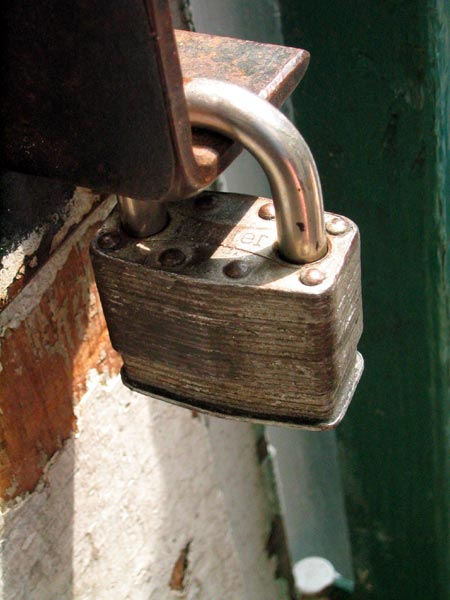
\includegraphics[width=0.5\textwidth]{images/padlock.jpg}

    \large What a real password protects --- exactly what a fake login page is built to steal.

    \small Padlock — Alyson Hurt, CC BY 2.0, via Wikimedia Commons
    \end{center}
\end{frame}

\begin{frame}{Let Them Discover}
    \Large
    Look closely at a real website address you trust. Could you design a lookalike version of it (swapping one letter for a similar-looking number)? Try writing one out on paper.
\end{frame}

\begin{frame}{Your Turn}
    \Large
    Open the student map, find \textbf{Computer Basics 4 — Phishing \& Fake Logins}, and work through it
    hands-on --- everything you just saw, they now do themselves.
\end{frame}

\end{document}
